% ═══════════════════════════════════════════════════════════
% §4 Results: Framework Characterization & Gap Attribution
% ═══════════════════════════════════════════════════════════
\section{Results: Framework Characterization}
\label{sec:results-characterization}

\subsection{Framework Comparison (RQ1)}

Unsloth BF16 achieves only a 5.2\% throughput advantage over HuggingFace native on consumer RDNA3 (129.4 vs 123.1 \toksec{} in the steady-state corrected caliber, Table~\ref{tab:framework}), far below the 2$\times$ speedup reported on data-center CDNA hardware. This modest gain is statistically significant (Welch's $t$-test, $p<0.01$, Cohen's $d>3$ across 3 seeds) but architecturally explainable: Unsloth's kernel fusion primarily eliminates intermediate memory round-trips, yet on RDNA3 the dominant bottleneck is compute throughput (WMMA instruction scheduling), not memory traffic. With 960 GB/s bandwidth already saturating the 3B-parameter model's weight loading, fusing operations yields diminishing returns.

The VRAM overhead tells a complementary story. Unsloth's 13.9\,GB footprint (vs 8.0\,GB for HF) reflects pre-allocated activation buffers and fused kernel workspaces that trade memory for compute efficiency. For the 3B model on a 24\,GB card this remains acceptable, but the 73.8\% overhead implies that scaling to 7B+ models will approach VRAM limits where HF's leaner allocation becomes necessary.

\begin{figure}[tbp]
\centering
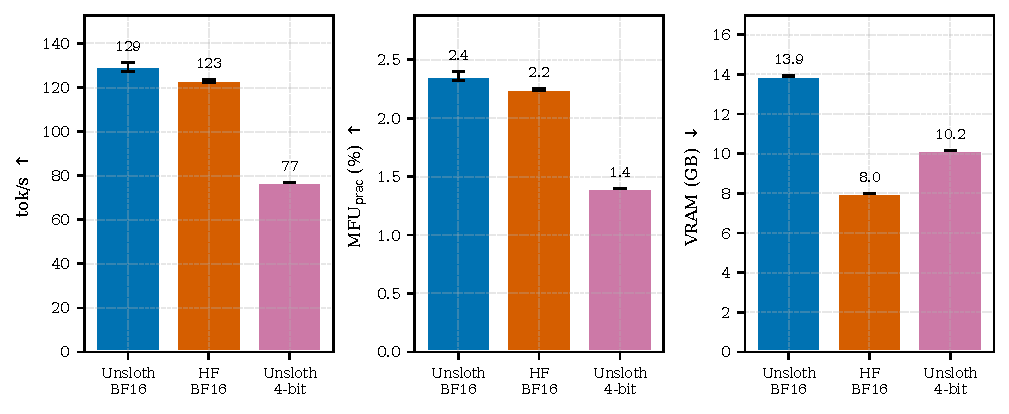
\includegraphics[width=\textwidth]{figures/fig_framework.pdf}
\caption{Framework comparison: throughput, MFU, and VRAM (3 seeds).}
\label{fig:framework}
\end{figure}

% Table 2: Framework efficiency comparison
% Fixed: reduced from 5 columns to 4, moved Valid to footnote
\begin{table}[t]
\centering
\footnotesize
\setlength{\tabcolsep}{4pt}
\caption{Framework efficiency comparison on GSM8K GRPO (steady-state corrected caliber).}
\label{tab:framework}
\begin{tabular}{@{}lccc@{}}
\toprule
\textbf{Framework} & \textbf{tok/s} $\uparrow$ & \textbf{\mfuprac} $\uparrow$ & \textbf{VRAM} \\
\midrule
Unsloth BF16 & 129.4$\pm$2.6 & 2.36$\pm$0.04\% & 13.9G \\
HF Native BF16 & 123.1$\pm$0.8 & 2.24$\pm$0.01\% & 8.0G \\
Unsloth 4-bit & 76.8 & 1.40\% & 10.2G \\
\midrule
\textit{Speedup (U/HF)} & \multicolumn{2}{c}{+5.2\%} & +73.8\% \\
\bottomrule
\end{tabular}
\end{table}


\subsection{4-bit Quantization: Architecture-Dependent Penalty}

NF4 quantization via BitsAndBytes~\citep{dettmers2023qlora} \textbf{reduces} throughput by 40.7\% on RDNA3 (76.8 vs 129.4 \toksec{}), a striking reversal of the memory savings that make QLoRA attractive on NVIDIA hardware. The mechanism is architectural: RDNA3 possesses no dedicated INT4 compute units, so every NF4$\rightarrow$BF16 dequantization before GEMM is pure overhead with no hardware acceleration. On NVIDIA A100, by contrast, 1248 TOPS of INT4 Tensor Core throughput absorbs dequantization cost within the compute pipeline.

Moreover, the VRAM ``savings'' are illusory on this workload: 10.2\,GB (4-bit) vs 13.9\,GB (BF16) represents only 27\% reduction, because the dominant memory consumer is activation storage and optimizer state, not model weights at 3B scale. The 41\% throughput penalty thus far outweighs a modest memory reduction. The practical implication is unambiguous: \textbf{on consumer RDNA3, always prefer BF16 over 4-bit quantization for training}.

\subsection{Efficiency Gap Attribution (RQ2)}

Component-stacking analysis (Table~\ref{tab:gap}, Figure~\ref{fig:waterfall}) reveals that the 97.7\% efficiency gap between GEMM peak and end-to-end GRPO training is overwhelmingly dominated by the inference stage: the L0$\rightarrow$L1 transition alone collapses utilization from 100\% to 0.23\% (a 101.3 TFLOPS loss). The four transitions yield distinct mechanistic insights:

\paragraph{L0$\rightarrow$L1 (Inference collapse).} Autoregressive decoding at batch size 1 has arithmetic intensity $\approx$1 FLOP/byte, placing it firmly in the bandwidth-bound regime. At 960 GB/s, each token generation reads the full 6\,GB model weight but performs minimal computation per byte loaded, leaving compute units idle.

\paragraph{L1$\rightarrow$L2 (Training recovery).} Batched training (batch\,=\,2, seq\,=\,256) restores arithmetic intensity through large GEMM operations in forward and backward passes. The recovered 27.2\% \mfuprac{} is comparable to reported LoRA fine-tuning MFU on data-center hardware~\citep{hu2022lora}, confirming that RDNA3's compute path is efficient once adequately loaded.

\paragraph{L2$\rightarrow$L3 (Checkpointing cost).} Gradient checkpointing imposes $-$26\% throughput (vs theoretical $-$33\% for one extra forward pass), because reduced memory pressure improves GPU cache utilization, partially offsetting recompute cost.

\paragraph{L3$\rightarrow$L4 (Generation domination).} End-to-end GRPO collapses to $\approx$2.3\% \mfuprac{} (estimated corrected caliber; see \S\ref{sec:statistics}) because the bandwidth-bound generation phase occupies the overwhelming majority of wall-clock time at small generation batch. The efficient training step (20--27\% \mfuprac{}) is diluted rather than amortized: with G=4 and per-device batch 1, tokens are generated at L1-like efficiency, then consumed by a brief high-efficiency update. This identifies generation batch scaling as the primary optimization target for RL post-training on this architecture.

\begin{figure}[tbp]
\centering
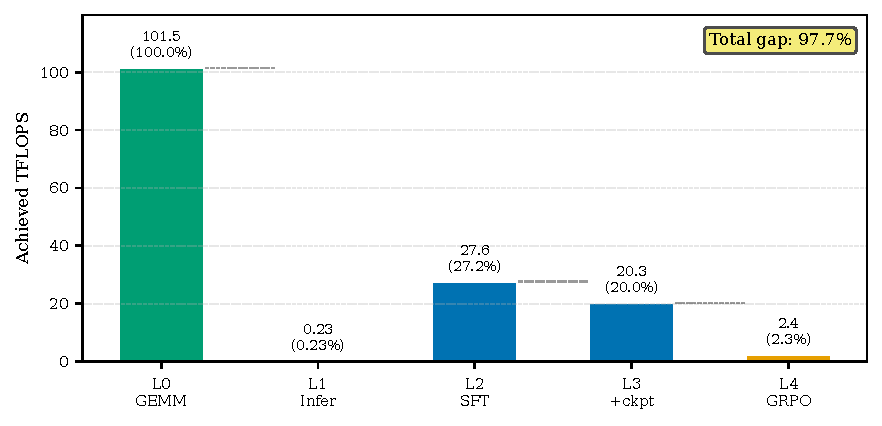
\includegraphics[width=0.85\textwidth]{figures/fig_waterfall.pdf}
\caption{Gap attribution waterfall. Inference (L1) dominates the total loss.}
\label{fig:waterfall}
\end{figure}

% Table 3: Gap attribution breakdown
% Fixed: shortened Mechanism column, footnotesize
\begin{table}[t]
\centering
\footnotesize
\setlength{\tabcolsep}{3pt}
\caption{Gap attribution breakdown with mechanistic explanations.}
\label{tab:gap}
\begin{tabular}{@{}lrrp{3.2cm}@{}}
\toprule
\textbf{Stage} & \textbf{TFLOPS} & \textbf{$\Delta$} & \textbf{Mechanism} \\
\midrule
L0: GEMM Peak & 101.53 & --- & Practical HW limit \\
L1: Inference & 0.23 & $-$101.3 & BW-bound (AI$\approx$1) \\
L2: SFT (no ckpt) & 27.63 & +27.4 & Batched F+B GEMM \\
L3: SFT (ckpt) & 20.33 & $-$7.3 & Recompute overhead \\
L4: GRPO Full & 2.35 & $-$18.0 & Gen-dominated wall-clock \\
\midrule
\textbf{Total Gap} & & \textbf{$-$99.2} & \textbf{97.7\% loss} \\
\bottomrule
\end{tabular}
\end{table}


The key insight for optimization: since the inference stage dominates the gap, any configuration that reduces generation's time share (shorter completions, higher G to amortize) will yield the largest throughput improvements. This directly motivates the tuning sweep in \S\ref{sec:results-tuning}.

\subsection{Summary}

Framework choice on consumer RDNA3 contributes a modest 5.2\% throughput difference, while 4-bit quantization is counterproductive. The dominant efficiency loss originates from autoregressive generation's bandwidth bottleneck, not from framework-level kernel efficiency. Hyperparameter choices that reduce generation overhead therefore offer far greater optimization leverage than framework selection, as we explore next.
